\chapter{Technology Trends}
\label{ch:trends}
Data center workloads have increased and diversified over the last decade. These changes are driven by emerging workloads such as artificial intelligence, big data and machine learning, but also by an increased demand of cloud services and a shift of compute from the edge of the network to the data center due to an increase in mobile devices. The following itemization summarizes different classes of workloads and examples \cite{stuecheli-power9, amd-epyc-datasheet, gupta-xeon}.

\begin{itemize}
  \item{Analytics: Big Data, High-Frequency Trading, and In-Memory Database.}
  \item{Cloud: Search, Virtualization, and Web Servers.}
  \item{Communication: Packet Processing and Virtual Switching.}
  \item{High Performance Computing: Artificial Intelligence, Genomics and Machine Learning.}
  \item{Security: Encryption and Decryption.}
  \item{Storage: Compression and Deduplication.}
\end{itemize}

%- “[Meanwhile], P. K. Gupta, the general manager of Xeon+FPGA products in Intel’s data center group, said FPGAs can increase the performance of applications such as machine learning, cloud radio-access networks, edge computing and content delivery. Accelerators can [also] increase performance at lower total cost of ownership for targeted workloads.”\\
%\url{https://www.rambus.com/blogs/the-role-of-fpga-acceleration-in-the-data-center-and-beyond-2/}\\

These changes in data center workloads demand not only more and faster resources (such as cooling, network and servers), but also a diversification of compute resources that can be dynamically tailored to the workload in question. Traditionally, servers consist of a fixed set of resources such as compute, memory, storage and I/O and are aggregated into a pool. Workloads are then scheduled on one or multiple pools. This architecture frequently results in under-utilization of resources due to a drastic real-time adjustment in available resources for specific workloads. This results in reduced power efficiency, or performance per Watt \cite{rambus}. The most important metric when building a new data center is the Total Cost of Ownership (TCO): the cost of purchasing and installing the hardware plus the cost to operate and maintain the data center over time. The electricity costs are roughly 15\% of the TCO \cite{research-cloud} and power consumption is becoming one of the most import metrics for data center operation and future hardware investments. Systems have to offer performance and power efficiency, while in the past performance was the dominant driver behind new investments. This makes Application Specific Integrated Circuits (ASICs), FPGAs and Graphics Processing Units (GPUs) more and more interesting due to their performance-to-Watt ratio.
%With reduced power efficiency, the data center operator pays for electricity to keep the server idle instead of doing useful work.

%OPTIMIZING DATA-CENTER TCO WITH SCALE-OUT PROCESSORS
%https://infoscience.epfl.ch/record/181904/files/tco_ieeemicro12.pdf

%A Simple Model for Determining True Total Cost of Ownership for Data Centers
%http://www.missioncriticalmagazine.com/ext/resources/MC/Home/Files/PDFs/(TUI3011B)SimpleModelDetermingTrueTCO.pdf





\section{Acceleration in the Data Center}
Traditionally, Moore's Law (which predicted exponential growth in the number of transistors on a chip) correlated well with single processor performance due to the increase in operating frequency that accompanied device scaling. The increase in the number of transistors per chip at a constant cost means that transistors become smaller and, if all dimensions are scaled, are able to switch at higher speeds. This explains the constant increase in frequency of processors until roughly 2006.





\subsection{Dennard Scaling}
In 1974, Dennard observed that the necessary current and voltage scale with transistor shrinking. This observation is known as Dennard scaling. Therefore, power consumption is proportional to transistor area. The total power consumed is the sum of dynamic and static power. Dynamic power is consumed by charging capacitors in the circuit and is shown in \autoref{eq:power}. Static power is consumed when the circuit is in quiescence.

\begin{equation}
  P = \alpha \times C \times F \times V^2, \text{where}
  \label{eq:power}
\end{equation}

\begin{itemize}
  \item{\textit{P} is the dynamic power,}
  \item{$\alpha$ is the percentage of time the circuit switches,}
  \item{\textit{C} is the sum of gate and wiring capacitance,}
  \item{\textit{F} is the frequency at which the circuit operates, and}
  \item{\textit{V} is the operating voltage of the circuit.}
\end{itemize}

% Original text talking about threshold voltage instead of gate oxide scaling.
% By shrinking transistors, capacitance and voltage can be reduced resulting in a higher operating frequency for the same dynamic power consumption. However, Dennard ignored two transistor parameters which define a baseline power consumption for a transistor: leakage current and threshold voltage. Leakage current is a phenomenon where charge carriers sip through the insulating region of a transistor, even in a rest state. Leakage current increases exponentially as the insulator thickness decreases, which occurs with the aggressive scaling of transistors. The voltage threshold is the minimum voltage required to establish a conducting path. With shrinking transistors, power density increased. Insufficient cooling capacity resulted in hitting the so-called \textit{Power Wall} in 2006 and limits processor frequency to around \SI{4}{\giga\hertz} \cite{dennard-scaling}.

However, \autoref{eq:power} involves simplified assumptions, because in the 1970's sub-threshold leakage was playing a relatively small role with respect to total power consumption. After several decades, sub-threshold leakage constrains further scaling of the threshold voltage and therefore also operating voltage. Due to leakage constraints, gate oxide scaling has also been affected. This prevents voltages from scaling as in the past, and thus starts to play a significant part in the total chip power. These factors limit the operating frequency of circuits \cite{mark-bohr}. Because voltages no longer scale, shrinking transistors now leads to power density increases. Insufficient cooling capacity resulted in hitting the so-called \textit{Power Wall} in 2006 that limits processor frequency to around \SI{4}{\giga\hertz} \cite{dennard-scaling}.

% From "A 30 Year Retrospective on Dennard's MOSFET Scaling Paper" by Mark Bohr from Intel.
% - But this 1974 work ignored the impact of transistor sub-threshold leakage on overall chip power. Sub-threshold leakage was relatively low in the 1970’s and was a tiny contributor to total power consumption on logic circuits. But after 30 years of scaling, VT has scaled to the point where sub-threshold leakage has increased from levels of <10-10 amps/mm to >10-7 amps/mm. Due to leakage constraints, it will be difficult to further scale VT and thus it will also be difficult to scale operating voltage.
% - Another key assumption in Dennard’s scaling law was the ability to scale gate oxide thickness. Gate oxide scaling has been a key contributor to scaling improvements over the past 30 years, but this trend is also slowing due to leakage constraints (see Figure 4). Intel’s 65nm generation transistors use a SiO2 gate dielectric with a thickness of 1.2 nm [2]. This dielectric is only about 5 silicon atomic layers thick and represents what is likely the limit to which SiO2 can be scaled. Not only are we running out of atoms, but gate oxide leakage due to direct tunneling current is becoming a noticeable percentage of overall chip power.





\subsection{Homogeneous Multi-Core Systems}
%In order to comply with performance and power efficiency requirements, workloads have to be mapped onto a compute resource which fits both requirements best. In a hierarchy of compute resources based on power efficiency, defined as performance per Watt, a CPU is on one side of the spectrum and an ASIC on the other. A GPGPU and FPGA fit in between these extremes respectively. In such a hierarchy, there is an inverse relationship between power efficiency and workload versatility.
%A CPU is the most versatile but has the worst power efficiency for certain workloads, while the function of an ASIC is fixed but is highly optimized for a specific task, therefore achieving better power efficiency. With such a diversity of workloads, it is obvious that not all workloads map entirely efficient to only a CPU or GPU. Some classes might have fine-grained parts which map efficiently to one, while the rest maps efficiently to another, or any other possible combination. Then there are also classes, or parts thereof, which map to neither.\\

Since 2006, after hitting the \textit{Power Wall}, and well before 2006 for server processors, Central Processing Units (CPUs) started to have multiple cores that work in parallel. Cores can be located within the same package, across multiple sockets, or across multiple systems. However, a workload across multiple homogeneous cores scales only as well as the portion of the workload that can be parallelized. Amdahl's Law \cite{amdahl}, shown in \autoref{eq:amdahl}, formulates the theoretical speedup of a workload when a portion of the system is improved and encapsulates this notion. The speedup is limited by the fraction of the task that does not benefit from the improvement. For example, if a task consists of one portion that can be parallelized and one portion that cannot, eventually the total latency is always bounded by the purely sequential portion.

\begin{equation}
  S_{latency}(s) = \frac{1}{(1-p) + \frac{p}{s}}, \text{where}
  \label{eq:amdahl}
\end{equation}

\begin{itemize}
  \item{$S_{latency}$ is the theoretical speedup of the workload at a fixed workload size, defined in latency,}
  \item{\textit{s} is the speedup of the portion of the workload that benefits from the improvement, and}
  \item{\textit{p} is the fraction of the execution time that \textit{s} initially occupied in the workload.}
\end{itemize}

%Using only homogeneous CPU cores limit the maximum speedup that can be achieved. Some workloads benefit from more cores than the current maximum of roughly 20. Multi-threading enables multiple virtual cores and increases parallelization further, but the total core count is well below 100.

A refinement to Amdahl's Law is Gustafson's Law \cite{gustafson}. This law takes into account that larger problems typically have a smaller sequential component.\\
The moment the energy to switch a single transistor does no longer decrease in a next process generation, using twice as many transistors to build twice the number of cores, only to have to turn off half of them because there is not sufficient power to feed them, is the end of the homogeneous multi-core era.





\subsection{Heterogeneous Multi-Core Systems}
\label{sec:hetero}
By applying a simple hardware model to Amdahl's Law, it is shown that a system with asymmetric cores can always achieve a higher maximum speedup than a system with homogeneous cores \cite{amdahl-era}. 
%Amdahl's Law implies that to speed up real workloads, consisting of serial and parallel portions, a heterogeneous system is required.\\
Typically, FPGAs and GPUs are used to improve parallel workloads, but in rare cases can also improve sequential workloads.\\

%\todo{PETER: interesting argument ... however, a GPU is usually thought to benefit only highly parallel workloads? ... the argument may be correct but is not an obvious one to make. -- If you argue for heterogeneous to address the fact that the sequential portion limits performance, then I think you need to argue explicitly that heterogeneous components can speed up sequential code, as people usually think that accelerators can only deal with the parallel portion. I do believe that our gzip accelerator is an example of speeding up code with many sequential dependencies.}

Arguably the most commonly used heterogeneous system in a nowadays' data center is a CPU-GPU system. In comparison to a CPU, a GPU consists of several thousands of cores operating at a frequency of roughly \SI{1}{\giga\hertz}. Dividing the workload between both compute resources is done manually, but yields a higher speedup compared to parallelization on CPUs only. Programming can be done in various languages but memory transfers between the CPU and GPU have to be invoked manually.\\

%due to the absence of a coherent shared memory space.
%An extreme case of multiple homogeneous cores is the currently widely adopted GPGPU, consisting of multiple thousands of cores. For example, a CPU-GPU system can be built where the serial portion of the workload is executed on the CPU while the parallel portion is executed on the GPU, resulting in a significant speedup. This decreases workload latency and improves power efficiency compared to a CPU-only or GPU-only system.
%"A Survey of CPU-GPU Heterogeneous Computing Techniques", ACM Computing Surveys, 47(4), 69:1--69:35, 2015

Similar to a homogeneous multi-core architecture found in GPUs, Intel released the Xeon Phi coprocessor. This coprocessor has a maximum core count and frequency of 72 and \SI{1.7}{\giga\hertz}, respectively, placing it in between a typical CPU and GPU \cite{phi}. The Xeon Phi can be considered as a GPU stripped from its typical graphics pipeline. Even with all these types of accelerators, there are workloads that do not benefit from the high operating frequency found in CPUs, nor the high core count found in GPUs or the Xeon Phi. Compute-intensive workloads that benefit from custom arithmetic units are an example.

%In the context of embedded systems, DSPs are specialized processors and often used to process input signals within a restricted power budget.\\

%\begin{figure}[H]
%  \centering
%  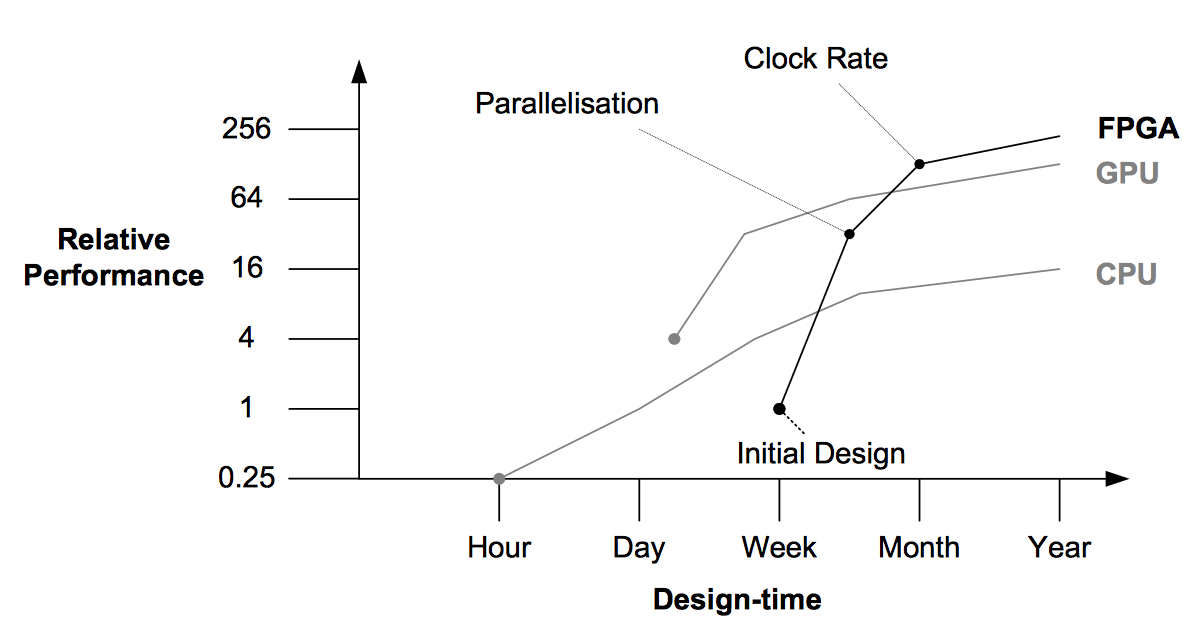
\includegraphics[width=0.70\textwidth]{1-cpu-gpu-fpga.png}
%  \caption{Illustration of relative performance versus the design time of several compute resources \cite{}.}
%  \label{fig:1-cpu-gpu-fpga}
%\end{figure}

%\autoref{fig:1-cpu-gpu-fpga} shows an illustration of the design time of workloads targeted at a CPU, GPU and FPGA versus the relative performance that can be achieved. After one day of development, the reference performance is obtained for the workload targeting a CPU after which it can slowly be improved upon. GPUs on the other hand take only slightly longer to design for, but immediately have large benefits in terms of performance. Finally, FPGAs are the most difficult to design for, since it consists both of hardware and software.
%\todo{- discuss two points in the graph}





\subsection{Application Specific Acceleration}
Two recent trends in the data center allow for a wider diversification of compute resources by introducing application specific accelerators in the form of ASICs and FPGAs.\\
One trend is to use fixed-function ASICs, either tightly coupled on-chip or loosely coupled using an interconnect. On-chip accelerators range from compression to cryptographic engines. An example of a loosely coupled accelerator is Google's recent Tensor Processing Unit (TPU) \cite{tpu}. While fixed-function ASIC accelerators provide a better power efficiency compared to a CPU and free up resources since the CPU is able to off-load work, on-chip accelerators consume valuable chip area while being dedicated to only one function. This renders a fixed-function accelerator useless when the underlying algorithm changes in the (near) future. Besides that, there are multiple time consuming steps in the design cycle of an ASIC that increase the time to market.\\
Another trend is the adoption of FPGAs. While FPGAs might not offer the same level of power efficiency that ASICs do, their (re)configurable nature allows for flexibility and reusability. According to the same study mentioned earlier \cite{amdahl-era}, reconfigurable or dynamic cores can always achieve a higher maximum speedup than asymmetric configurations. While the design cycle of ASICs can be up to several years, FPGAs can be designed in a fraction of that time because layout and fabrication are not required. However, FPGAs are more difficult to use compared to CPUs and GPUs since both hardware and software have to be developed. FPGAs have not invested as heavily in double-precision floating-point pre-integrated units. Therefore they specifically shine in non-floating point compute-intensive workloads, on parallel workloads because of their inherently parallel architecture, and also in network communication related acceleration. Parallelism can be exploited at different levels of granularity and optimized fixed-function hardware accelerates the compute-intensity. %They also have a high IO pin count.
The downside is that an FPGA consists of various pre-defined resources, like memories and DSP slices, that constrain the degrees of freedom of the design. When deployed as a compute accelerator FPGAs have typically been connected using a relatively low-bandwidth and high-latency interconnect, limiting their use for memory-intensive workloads. When deployed as network switches, FPGAs have typically been deployed with very high bandwidth using leadership PHYs (Physical Layers).





\subsection{FPGA Adoption in the Data Center}
\label{sec:adopt}
FPGAs are becoming more interesting for specific workloads in the data center for various reasons. The (re)configurability allows for reuse and on-the-fly adaptation.
%, FPGAs have been shown to outperform other types of compute resources in terms of operations per byte for specific workloads. 
In addition, FPGAs are more power efficient than other compute resources. This aspects becomes increasingly important for data center operators to keep the TCO down. Traditional limitations of FPGAs are starting to fade away with recent advancements in interconnect standards and system design.

\begin{itemize}
  \item{\textbf{Interconnect limitations}, such as low bandwidth and high latency, limit FPGAs to parallel and latency-insensitive workloads, because latency of the interconnect is much higher than that of host memory. Upcoming interconnect standards target these limitations.}
  \item{\textbf{Programmability} is limited to the use of hardware description languages. Advancements in software frameworks and high-level language to HDL compilers make FPGA acceleration accessible to software engineers. Also manual data movement between the CPU and FPGA is error prone and slow due to copy operations through memory and driver overhead. The typical off-load programming model is being replaced by a shared memory model with advancements in system design. This enables seamless integration of FPGAs with CPUs and lets the FPGA act as a thread-level functional unit instead. Accessing FPGAs for development becomes simpler by using cloud platforms such as Amazon EC2 F1.}
\end{itemize}

%Traditionally, FPGAs were applied to parallel and latency insensitive workloads, because latency of the interconnect is much higher than that of main memory. This is changing with upcoming interconnect standards such as CCIX, OpenCAPI and PCI Express gen 4.

%Also advancements regarding programmability are enabling adoption. The typical off-load programming model is being replaced by a shared memory model due to advancements in interconnects. This enables seamless integration of FPGAs with CPUs and lets the FPGA function as a thread-level functional unit instead of as an off-load engine.
%Finally, software frameworks have dramatically improved. No longer is the knowledge of an HDL needed, since multiple high-level language to HDL compilers exist. Examples are HLS by Xilinx, Matlab, Haskell, OpenCL, etc. A special framework is SNAP for CAPI 1.0, which extends the interconnect with a simplified API and easily integration of the accelerated function. Another initiative is the Vineyard project, which lets the compiler decide on which compute resource to use, provided that the requested accelerated function is available in their database.

One approach is integration of CPUs with FPGAs, like Intel is doing with their Xeon processors \cite{gupta-xeon}. The FPGA is currently on the same package as the CPU and expected to be on the same die in the future. Such advancements enable a high bandwidth interconnect. Another approach is by using off-chip interconnects to attach FPGAs. We are interested in the latter approach, since such advancements in interconnects are also beneficial for other attached devices.

% The first problem is addressed by a large number of available compilers and frameworks which convert (parts of) higher-level programming languages to HDL. Examples include MatLab HDL Coder, Xilinx HLS for C, C++ and SystemC, CLaSH for Haskell to HDL, OpenCL for C and C++, Reconfigure for Go to HDL and MyHDL for Python to HDL. The attainable performance of these tools might not achieve similar performance as fully custom FPGA designs.

%FROM FRONTIERS PDF chapter 1\\
%This adoption is two-fold. First of all, software stacks to program FPGAs have greatly evolved and nowadays also allow for high-level languages to compile into HDL. Second of all, it becomes more difficult to extract performance out of multi-core CPUs. Small performance jumps are made in every generation, mostly by improving the throughput, but not the single-core performance. REF FRONTIERS\\
%But both FPGA and GPU accelerators offer a more compelling improvement in performance per watt. Hybrid CPU-FPGA and CPU-GPU systems can offer similar performance and performance per watt, at least according to tests that Microsoft has ran, on deep learning algorithms. The GPUs run hotter, but they do roughly proportionally more work and at the system level, offer similar performance per watt.\\
%FPGAs have had a notorious reputation for a long time. They were difficult to program and set up and required an expert to do so. Also the scarce availability of logic resources and memory capacity per card and slow interconnect resulted in only being applicable to specific workloads. Therefore the FPGA was only used in a niche market.\\
%From machine learning, high performance computing, data analytics, and beyond, there is a new day dawning for FPGAs in a more diverse range of application areas. Highly parallel workloads that ca be contained in a small power envelope and take advantage of the growing amount of on-chip memory available on FPGAs are all in the sights of FPGA makers and potential end users.\\
%fpgas can battle for ML with gpus because of their power envelope. however a better fit is cloud computing, but programming difficulty is holding it back.\\
%FPGAs are set to become a companion technology in some hyperscale datacenters, Dhulla says. “We are seeing that these datacenters are separated into ‘pods” or multiple racks of servers for specic workloads. For instance, some have pods set aside to do things like image resizing, as an example. Here they are  nding a  t for FPGAs to accelerate this part of the workload.” In other hot areas for FPGAs, including machine learning, Dhulla says that they are operating as a “cooperating” accelerator with GPUs. “There is no doubt that for the training portion of many machine learning workloads GPUs are dominant. There is a lot of compute power needed here, just as with HPC, where the power envelope tradeoff is worth it for what is required.”\\
%fpgas are very much adopted in financial market due to their good integer performance\\
%seems like fpgas are being used as the glue between the cpu and the gpu. to accelerate very specific parts of a workload.\\
%Over the last year there have been a few highly publicized use cases highlighting the role of FPGAs for specific workloads, particularly in the deep learning and neural network spaces, as well as image recognition and natural language processing. For instance, Microsoft used FPGAs to give its Bing search service a 2X boost across 1,632 nodes and employed a creative 2D torus, high throughput network to support Altera FPGA-driven work. China’s search engine giant, Baidu, which is also a heavy user of GPUs for many of its deep learning and neural network tasks, is using FPGAs for the storage controller on a 2,000 petabyte array that ingests between 100 terabytes to a petabyte per day. These and other prominent cases of large-scale datacenters using FPGAs, especially when they do so over GPUs, are bringing more attention to the single- precision  oating point performance per watt that FPGAs bring to the table.\\
%While some use cases, including the Baidu example, featured GPUs as the compute accelerator and FPGAs on the storage end, Altera, Xilnix, Nallatech, and researchers from IBM on the OpenPower front were showcasing where FPGAs will shine for deep learning in the cloud. The takeaway from these use cases is that the speedups for key applications were hosted inside ultra-dense machines that would melt the Xeon if a GPU was placed in concert. For tight-packed systems, they are a viable choice on the thermal front and even though there might not be as many algorithms where FPGAs can show off (compared to GPUs) this could be the beginning of a golden era for the coprocessors, especially now that there are CAPI and QPI hooks for taking advantage of shared memory on FPGA-boosted systems.\\
%If you ask Altera, Xilinx, and others, this is happening because of what we can call the “three P’s of FPGA adoption” – performance, power, and price. In early 2016, we were able to sync up with several of the main FPGA vendors at the GPU Technology Conference (the irony) and co-located OpenPower Summit, where we heard quite a bit about the golden age of the FPGA—all brought about by the cloud. With an estimated 75 percent of all servers being sold to live a virtualized life, the market rationale is not dif cult to see—but performance per watt is the real story, especially when compared to GPUs, says Mike Strickland, who directs the compute and storage group at Intel/Altera. That puts Strickland in direct contact with HPC and hyperscale shops and gives him an understanding of their architectural considerations.\\
%Although FPGAs have the reputation of being expensive, at high volume they are on par with other accelerators, Strickland explained, pointing to Microsoft as a key example. However, he says that the ef ciencies of the performance boost far outstrip GPUs for neural algorithms, which leads to additional savings. There are numerous charts and arts highlighting the price/performance potential of FPGAs in both bare metal and virtual environments, but the real question is that stubborn fourth “P’ – programming.\\





\section{Interconnect Trends}
In this section, the two typical drawbacks of FPGA adoption are explored in more detail. First bandwidth trends are explored, followed by reported improvements in FPGA programmability. Software framework and high-level to HDL compiler advancements are not discussed further in this thesis.



\subsection{Attached Devices Push Bandwidth Requirements}

%- network: find study of what percentage of network bw is used by which applications.\\
%- network: besides ethernet bw increasing from 10, to 100 to soon 400 Gb/s, how does inifiniband and others fit in? Infiniband is only within or between servers. Not like ethernet.\\

Besides the adoption of various kinds of accelerators in the data center, the balance of bandwidths at system-level have changed significantly in recent years. Advancements in networking and storage result in increased bandwidth requirements of such devices. With the increase in complexity and volume of data center workloads, there is never enough or fast enough storage available. 
Emerging workloads, such as big data and machine learning, using data sets in the order of exabytes ($10^{18}$), are good examples of this \cite{teradata}.
%According to EMC\textsuperscript{2}, by 2020 about \SI{1.7}{\mega\byte} of data will be created every second per human \cite{big-data}. 
Therefore, new storage protocols are quickly adopted, with NVMe over PCI Express being the latest achieving bandwidths of several gigabytes per device. The previous generation reached only half a gigabyte at best. Network bandwidths are increasing similarly by quick adoption of both the \SI{100}{\giga\bit\per\second} and \SI{400}{\giga\bit\per\second} standards in only a few years time. With more and more data and services moving to the cloud, network bandwidths have to increase rapidly.



\subsection{Bandwidth Trends at Device-Level}
Fritz Kruger, a SanDisk Fellow, collected data regarding DRAM, network and storage bandwidth for a presentation in 2016 and predicted the future until 2020. \autoref{fig:1-fritz} shows his findings, with the addition of PCI Express bandwidth to act as a proxy for interconnect bandwidth. For each generation of the PCI Express standard, the bandwidth of sixteen lanes is plotted, since this is typically the maximum number of lanes per PCI Express device. DRAM is inherently uni-directional and several cycles are required to turn the channel around. A memory controller takes care of this by combining reads and writes to limit the overhead cycles spent in configuring the channel. Therefore, DRAM bandwidth should be interpreted as either a read or write channel with the plotted bandwidth, while attached devices such as network and storage typically have a bi-directional link.\\
The slope of each of the fitted lines is important here. Clearly, both network and storage bandwidths are increasing at a much faster rate (steeper slope) than DRAM and PCI Express. The network and storage slopes are similar and double every 18 months. PCI Express doubles every 48 months while it takes DRAM 84 months to double in bandwidth. A shift in system balance is expected for future systems where DRAM, interconnect, network and storage bandwidth are about the same.\\
The fitted straight lines for each of the four data sets shown in \autoref{fig:1-fritz-bw-log} indicate exponential behavior, which can be clearly seen in \autoref{fig:1-fritz-bw}. This figure shows exactly the same data, but on a linear y-axis instead. While it might look like accelerators, such as GPUs and FPGAs, will have to compete for interconnect bandwidth with network and storage, vendors can always scale memory and interconnect bandwidth accordingly. While scaling is the trend, as becomes apparent from the next paragraph, and works in the short-term, it does not solve the fundamental problem of lacking DRAM bandwidth improvements.\\
The reason that DRAM bandwidth is not increasing at a similar pace is two fold. Typically, the number of channels or the channel frequency is increased. However, each solution has significant implications. Every additional channel requires a large number of pins (order of 100) on the processor package (assuming an integrated memory controller) that increases chip area cost. Increasing channel frequency requires expensive logic to solve signal integrity problems at the cost of area, and more aggressive channel termination mechanisms at the cost of power consumption \cite{dram-1, dram-2}.
%- Why does DRAM bandwidth not double faster? Capacity scaling problem is known (DRAM technology limitations). Question at IBM ARL talk.\\

%\todo{- [Style] Even out subfigure width.\\
%- [Ask] Fit straight line on fig a and exponential curve on fig b.\\
%- [Peter] DRAM and SATA are half-duplex while PCI Express and Ethernet are full-duplex. How to compare?\\ Plotted PCI Express interconnect as uni-directional. Change plot axis names accordingly.\\
%}

%\begin{figure}[H]
%  \begin{subfigure}{0.5\textwidth}
%    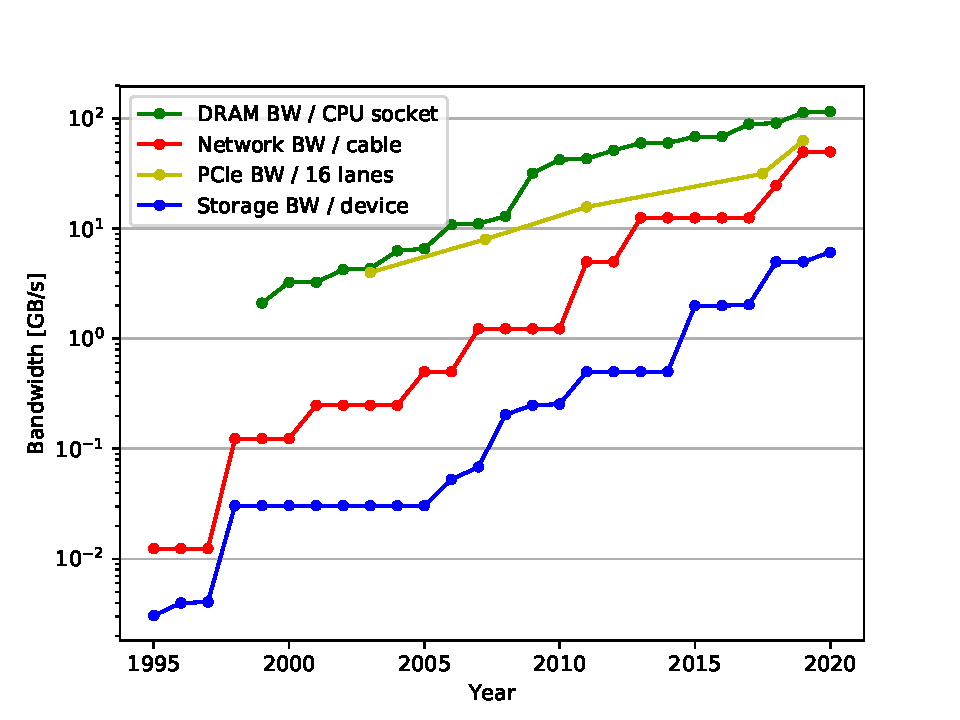
\includegraphics[width=1.0\linewidth]{1-fritz-bw-log.pdf}
%    \caption{Data plotted on a semi-log scale.}
%    \label{fig:1-fritz-bw-log}
%  \end{subfigure}
%  \begin{subfigure}{0.5\textwidth}
%    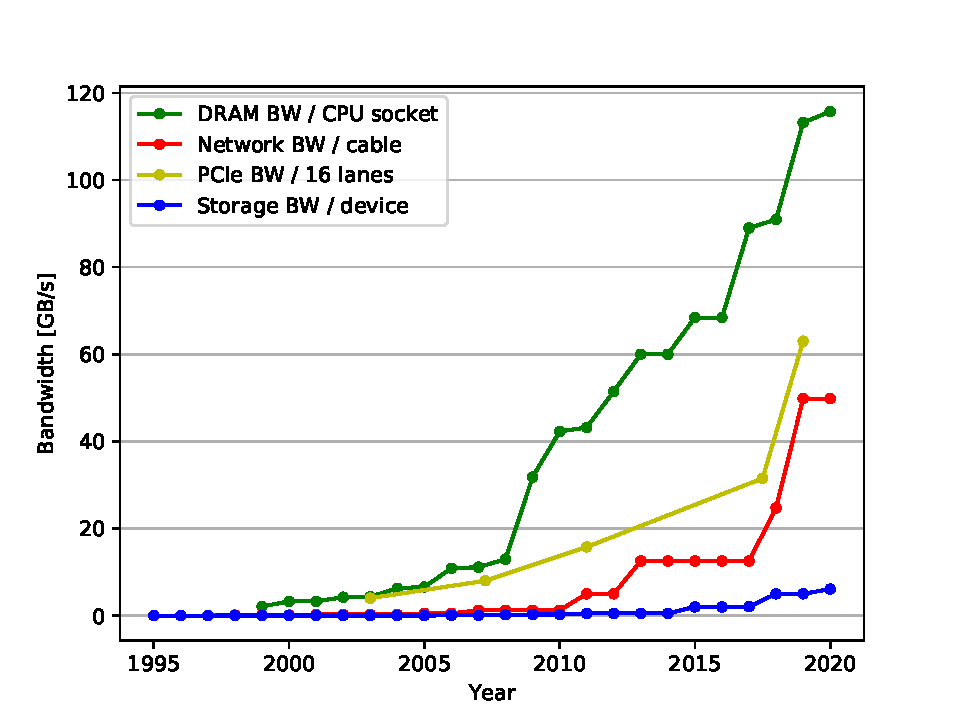
\includegraphics[width=1.0\linewidth]{1-fritz-bw.pdf}
%    \caption{Data plotted on a linear-linear scale.}
%    \label{fig:1-fritz-bw}
%  \end{subfigure}
%  \caption[Bandwidth at device-level trends Fritz reference.]{Bandwidth trends at device-level \cite{fritz}\footnotemark.}
%  \label{fig:1-fritz}
%\end{figure}

\begin{figure}[htb!]
\ffigbox[\textwidth]
  {
    \begin{floatrow}
    \ffigbox[\linewidth]
      {\captionof{subfigure}{Data plotted on a semi-log scale.}
      \label{fig:1-fritz-bw-log}}
      {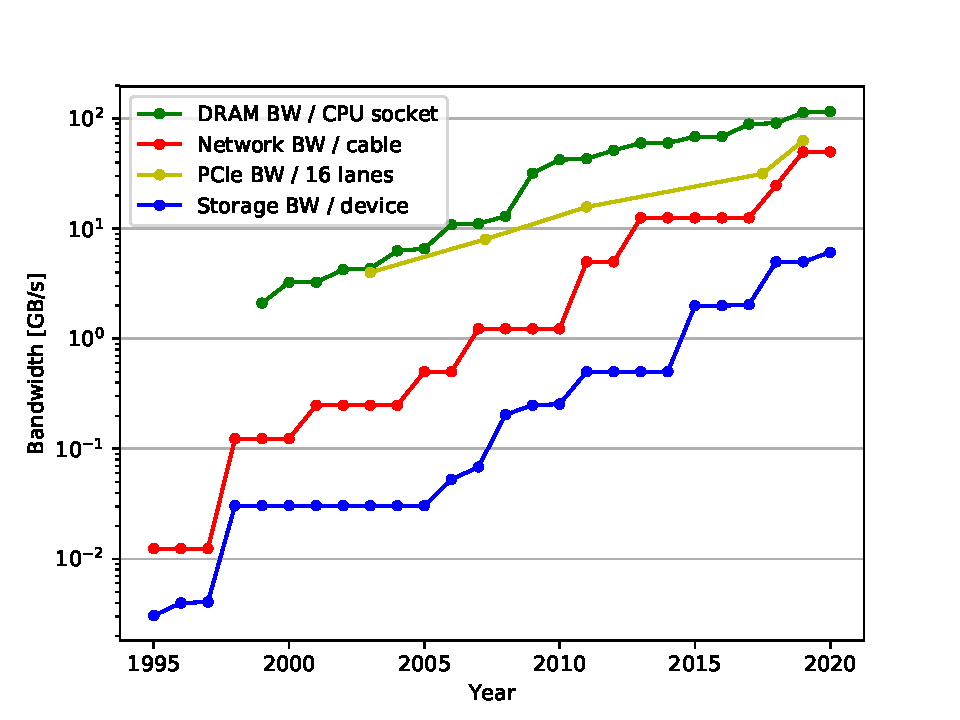
\includegraphics[width=1.0\linewidth]{1-fritz-bw-log.pdf}}
    \ffigbox[\linewidth]
      {\captionof{subfigure}{Data plotted on a linear-linear scale.}
      \label{fig:1-fritz-bw}}
      {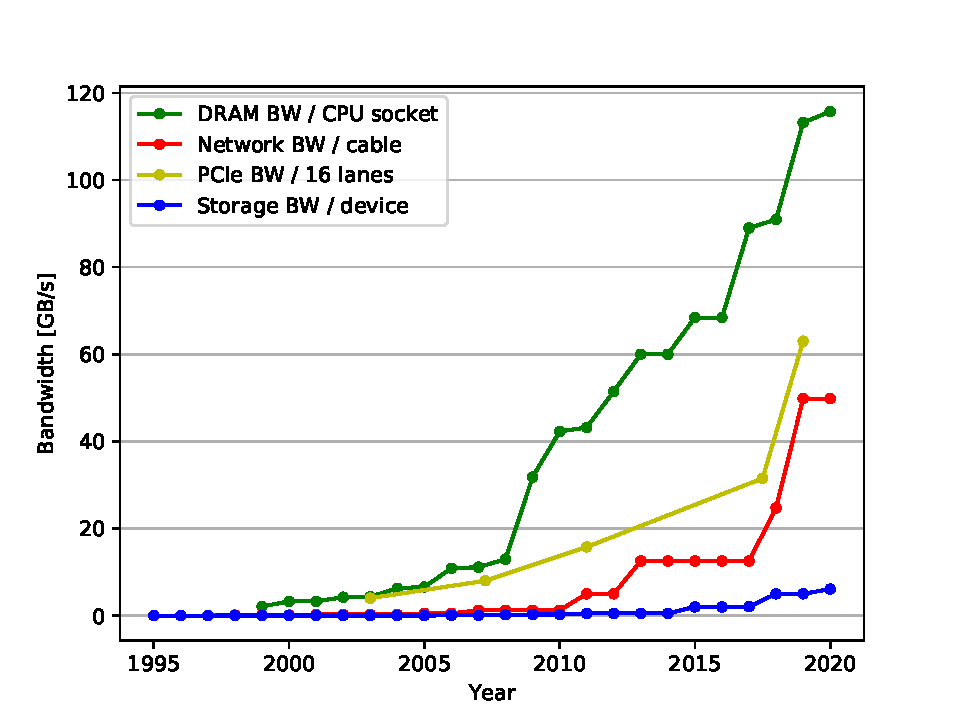
\includegraphics[width=1.0\linewidth]{1-fritz-bw.pdf}}
    \end{floatrow}%
  }
  {\caption[Bandwidth at device-level trends Fritz reference.]{Bandwidth trends at device-level \cite{fritz}\footnotemark.}\label{fig:1-fritz}}
\end{figure}
\footnotetext{Data points were approximated from the referenced figures in order to add the PCI Express standard bandwidth and represent all bandwidths in GB/s.}



\subsection{Bandwidth Trends at System-Level}
\label{sec:bw-trends}

%\todo{- [Ask] Finish bandwidth plots.\\
%- [Extra] SPARC CPU info\\ %\url{https://nl.hardware.info/nieuws/53488/oracle-introduceert-sparc-m8-database-processor}\\
%}

In order for vendors to stay ahead of the inevitable crossing of DRAM, interconnect, network and storage bandwidths, scaling is applied to both DRAM and interconnect bandwidth for the short-term. While the previous figures show predictions for future generations, more recent information regarding upcoming or recently released CPUs indicate that there is a large push to more DRAM and interconnect bandwidth. \autoref{fig:1-processor-bw} shows the peak\footnotemark~DRAM and interconnect bandwidth per CPU generation for single socket systems over a span of eight years. Per vendor and generation, the highest rated model is shown. Note that in the case of Intel, the E5 models have more interconnect bandwidth, while the E7 models have more DRAM bandwidth. Unreleased CPUs are plotted at the year 2018.

\footnotetext{The only exception are the IBM POWER8 and POWER9, which state the sustained DRAM bandwidth.}

%\begin{figure}[H]
%  \captionsetup[subfigure]{justification=centering}
  %\centering
%  \begin{subfigure}{0.5\textwidth}
%    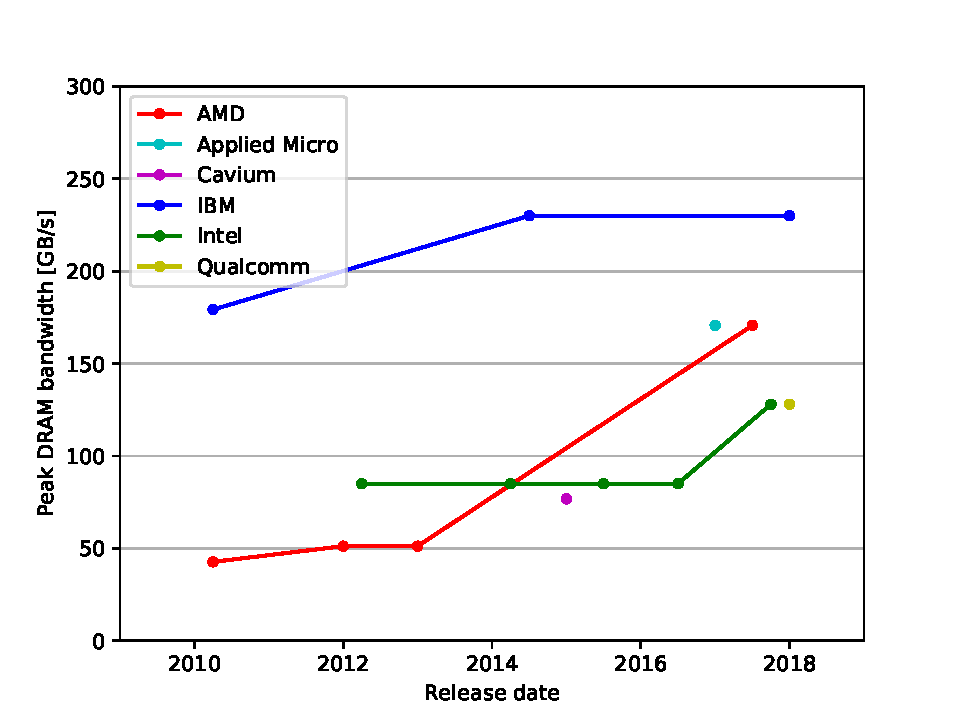
\includegraphics[width=1.0\linewidth]{1-processor-bw-dram.pdf}
%    \caption{Peak DRAM bandwidth.}
%    \label{fig:1-processor-bw-dram}
%  \end{subfigure}
%  \begin{subfigure}{0.5\textwidth}
%    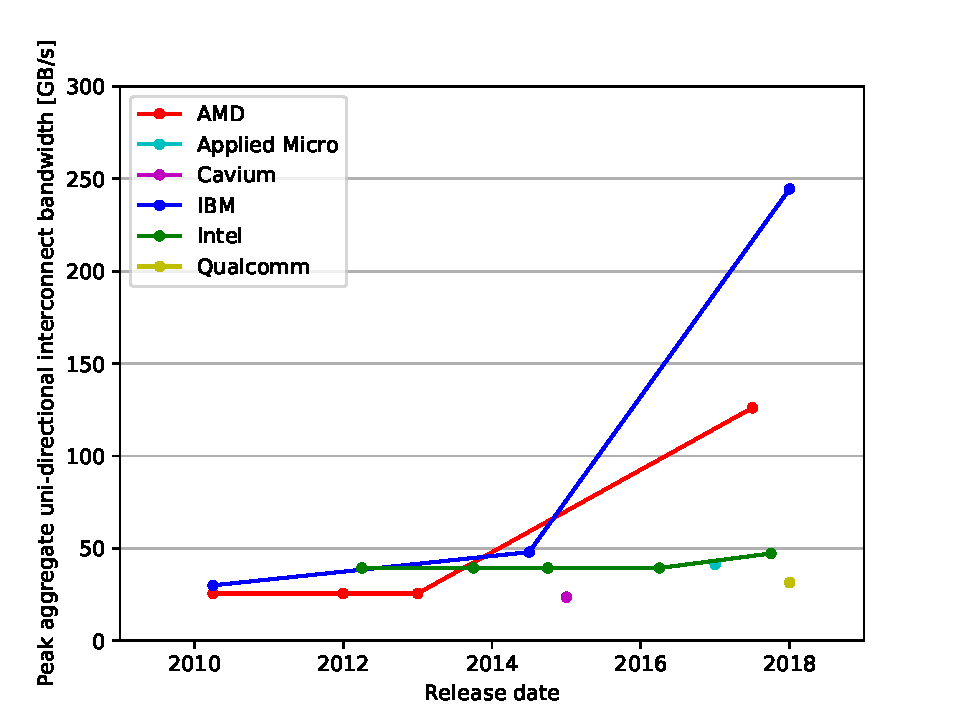
\includegraphics[width=1.0\linewidth]{1-processor-bw-io.pdf}
%    \caption[Peak aggregate uni-directional interconnect bandwidth.]{Peak aggregate uni-directional\\interconnect bandwidth.}
%    \label{fig:1-processor-bw-io}
%  \end{subfigure}
%  \caption{Study of bandwidth trends at system-level for single socket CPUs per generation.}
%  \label{fig:1-processor-bw}
%\end{figure}

\begin{figure}[htb!]
\ffigbox[\textwidth]
  {
    \begin{floatrow}
    \ffigbox[\linewidth]
      {\captionof{subfigure}{Peak DRAM bandwidth.}
      \label{fig:1-processor-bw-dram}}
      {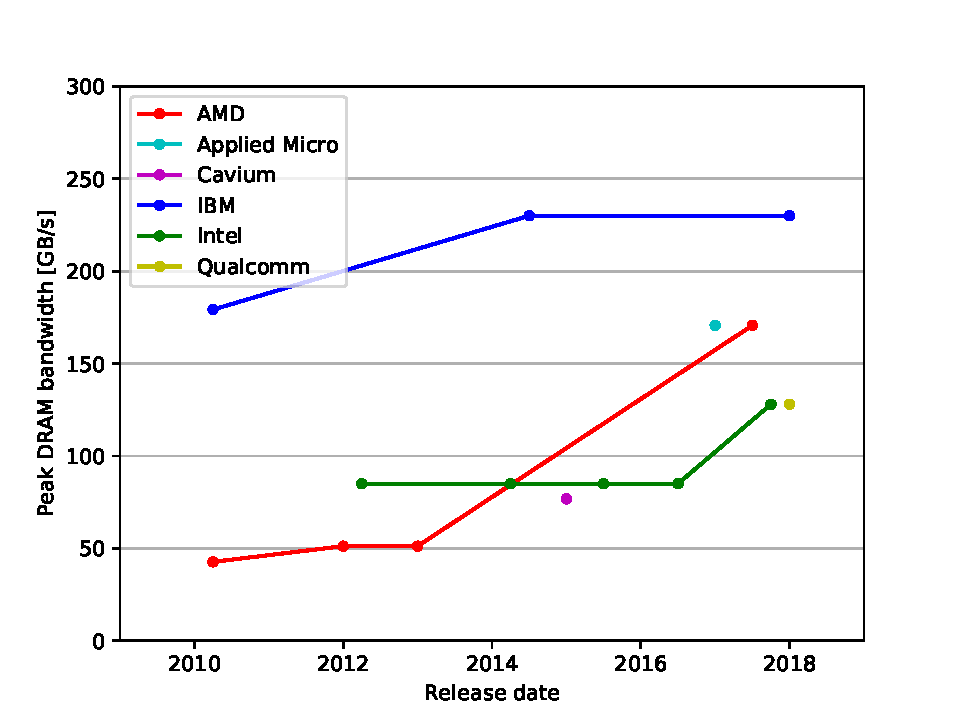
\includegraphics[width=1.0\linewidth]{1-processor-bw-dram.pdf}}
    \ffigbox[\linewidth]
      {\captionof{subfigure}{Peak aggregate uni-directional interconnect bandwidth.}
      \label{fig:1-processor-bw-io}}
      {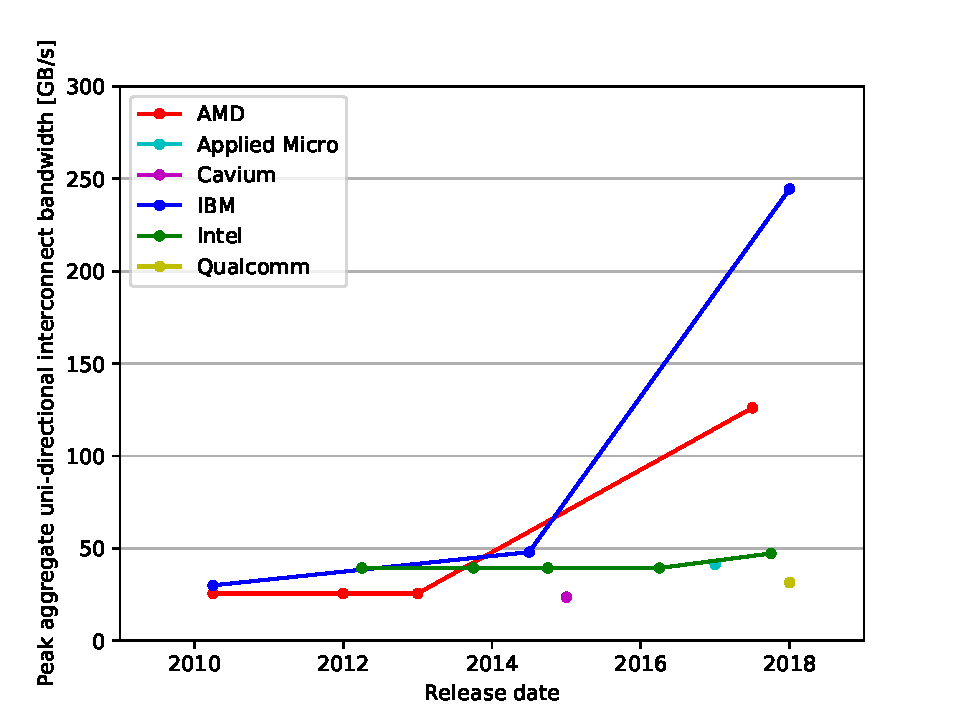
\includegraphics[width=1.0\linewidth]{1-processor-bw-io.pdf}}
    \end{floatrow}%
  }
  {\caption{Study of bandwidth trends at system-level for single socket CPUs per generation.}\label{fig:1-processor-bw}}
\end{figure}



\subsubsection{DRAM Bandwidth Trends}
The DRAM bandwidth data shown in \autoref{fig:1-fritz} was mostly taken from the Intel Xeon product family according to the author \cite{fritz}. \autoref{fig:1-processor-bw-dram} shows that AMD and IBM, compared to Intel, scaled their DRAM bandwidth aggressively by increasing the number of memory channels or by using additional buffer chips between the last-level cache and the DRAM. Only after several years did Intel improve the memory bandwidth in their latest generation by increasing the operating frequency and number of channels. While the Intel Xeon DRAM bandwidth follows the predictions quite well, both AMD's EPYC processors and IBM's POWER8 and POWER9 processor break the trend. The POWER processors offer roughly twice as much memory bandwidth compared to the latest Intel Xeon family.\\
An implication for the slow DRAM bandwidth increase is that flash storage can be attached as accelerator and act as DRAM or local storage for a data intensive accelerator, for example by exploiting data locality.



\subsubsection{Interconnect Bandwidth Trends}
\autoref{fig:1-processor-bw-io} shows the peak aggregate uni-directional interconnect bandwidth per CPU socket. This is calculated as the product of the uni-directional bandwidth per lane and the number of lanes. In the past, nearly every vendor used their own interconnect standard, possibly with a bridge to PCI Express. The general consensus is to use PCI Express and it has become the industry standard. While the introduction of PCI Express Gen 4 took longer than previous generations (see \autoref{fig:1-fritz-bw-log}), initiatives took off to extend the PCI Express standard with coherency protocols for seamless integration of attached devices. IBM started in 2014 with CAPI and more recently the CCIX consortium tries to implement a protocol for current and future PCI Express standards.\\
The aggregate interconnect bandwidth at system-level is increasing by an order of magnitude and has passed DRAM bandwidths. In the latest generation, both AMD and IBM are investing aggressively. AMD scaled the number of PCI Express Gen 3 lanes per socket to 128 lanes. For comparison, the latest Intel processor offers a maximum of 48 lanes for the same PCI Express generation. However, for multi-socket systems the AMD CPU will sacrifice half of its lanes for SMP, while Intel has a dedicated link for that. IBM's upcoming POWER9 processor has almost twice the interconnect bandwidth compared to AMD. This is achieved by having 48 lanes of PCI Express Gen 4 and 48 lanes of a new \SI{25}{\giga\bit\per\second} link called BlueLink. Note that both types of interconnect on the POWER9 can be used for SMP as well. This fundamental improvement enables a massive increase in bandwidth compared to other state-of-the-art systems. Although a significant improvement, it is only a small bump on the log-scale in \autoref{fig:1-fritz-bw-log}.\\
Very recently, new players such as Applied Micro, Cavium and Qualcomm are entering the server processor market with ARM-based processors. Such servers are targeted for cloud, content delivery, storage and web workloads and differ greatly from the traditional high performance and power consuming POWER and x86 architectures. These types of workloads do not require high-bandwidth accelerators, but instead prefer fixed-function on-chip accelerators and integrated network adapters. This class of servers does allow for memory bandwidths similar to those of Intel.

This study shows that the latest generation of processors tries to keep up with the exponentially increasing bandwidth of network and storage by scaling the interconnect in a similar fashion, and no longer follows the tradition shown in \autoref{fig:1-fritz}. It is important that DRAM bandwidth scales as well, in order to not become a bottleneck. Increasing the interconnect bandwidth by an order of magnitude forces us to reconsider design choices for accelerators.





\section{Current Interconnect Bottlenecks}
\label{sec:current}
It has been shown that an increase in interconnect bandwidth is required for emerging workloads in the data center. However, this problem is not solely solved by blindly scaling the current interconnects because the traditional Input/Output (IO) model will become a bottleneck. This section introduces the traditional IO model and its bottlenecks.

%\todo{- [Extra] Explain difference between memory and IO mapped devices. See comments.\\ %Nice picture: \url{https://www.robots.ox.ac.uk/~dwm/Courses/2CO_2014/2CO-N4.pdf}. main point is io mapped is in separate address space (x86 IN and OUT instructions), while memory mapped is in same address space. currently mostly used, io mapped is more for embedded.\\
%}



\subsection{Traditional IO Model}
\label{sec:copies}
Workloads contain serial and parallel components, where parallel components typically benefits from highly parallel architectures as mentioned in Section \ref{sec:hetero}. Due to the need for heterogeneous systems, different compute elements must communicate efficiently without decreasing potential execution speedup.\\
In a traditional IO model, the host processor has a shared memory space across its cores with coherent caches. Attached devices such as FPGAs, GPUs, network and storage controllers are memory-mapped and use a DMA to transfer data between local and system memory across an interconnect such as PCI Express. Attached devices can not see the entire system memory, but only a part of it. Communication between the host processor and attached devices requires an inefficient software stack in comparison to the communication scheme between CPU cores using shared memory.\\
\autoref{fig:2-memcpy} shows the data flow in the traditional IO model. The yellow boxes within the purple physical memories indicate seperate address spaces. In order to offload data from host memory to an attached device, data is copied from the application (\textit{app}) region by the CPU into a pinned (non-pageable) section of the host memory called a buffer. Only the buffer is visible to the attached device (due to different address spaces, therefore different instructions for memory and Memory Mapped IO (MMIO) accesses), because it does not share the same translation tables with the CPU. By reading the buffer, with the help of device drivers, the CPU is able to write the data, across an interconnect, into the local memory of the attached device. The attached device fulfills a certain \textit{Function}, which reads the data from the local memory and processes it. The result will then be written into the local memory after which the \textit{Function} informs the host it has finished. A DMA for example will move the result into a second buffer within the host memory. From here, the CPU copies the data to the application address space after which the application can continue.

\begin{figure}[H]
  \centering
  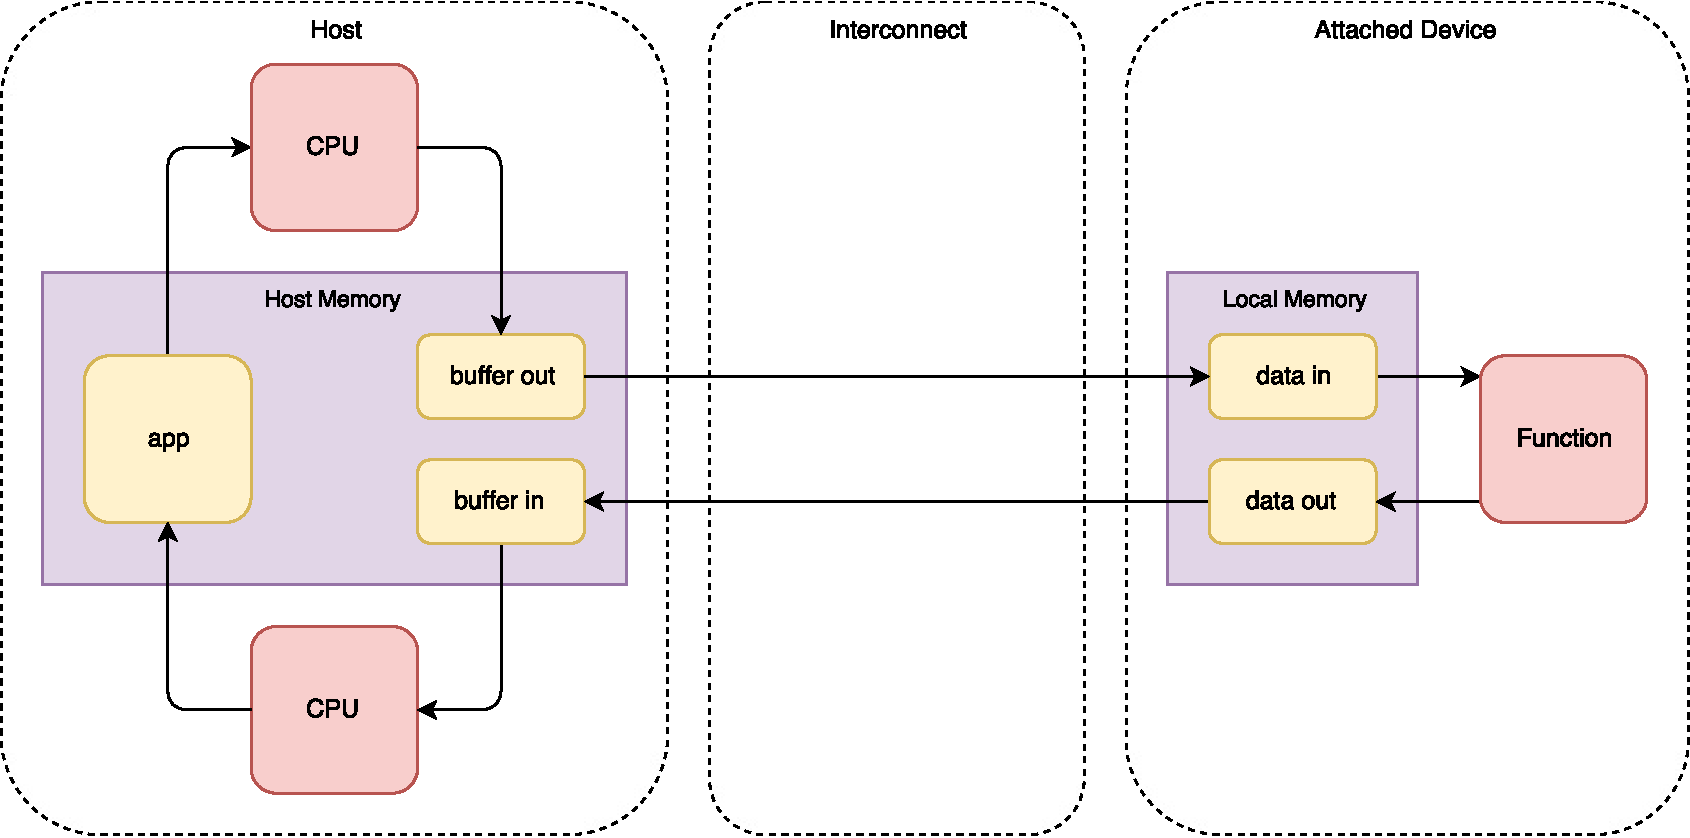
\includegraphics[width=0.80\textwidth]{2-memcpy.pdf}
  \caption{Multiple copy operations in the traditional IO model.}
  \label{fig:2-memcpy}
\end{figure}



\subsection{Communication and Synchronization Overhead}
Communication and synchronization between the host and attached device using interrupts and MMIO operations typically involves the device driver and introduces overhead \cite{capi-zurich}. These communication channels are used to start or stop the attached device.\\
While the attached device is operational, typically the \textit{app} running on the host is idle and waits for the \textit{Function} to finish, after which they synchronize and continue.\\
Functions with a relatively low number of data transformations suffer from a high interconnect overhead per data element with the traditional model. The communication overhead decreases the potential execution speedup, limiting acceleration to data transformation intensive workloads.



\subsection{Host Memory Access Congestion}
Another bottleneck, illustrated by \autoref{fig:2-memcpy}, is the host memory bandwidth for systems with increasing interconnect bandwidth such as the ones shown in Section \ref{sec:bw-trends}. The traditional model requires four memory copy operations, of which the CPU is involved in a total of three reads and two writes across the host memory channel. Since all attached devices can potentially use all of their assigned bandwidth, the host memory channel will suffer from severe congestion for servicing all copy operations. The fact that host memory is inherently simplex and cycles are required to turn the channel around is not beneficial either.



%\subsubsection{Case Study: Intel Xeon Gold 6154}
%To illustrate this problem, \autoref{fig:2-system-1} shows a hypothetical system where host memory, an accelerator (ASIC, FPGA or GPU) and a network and storage controller are attached to the CPU. With the traditional IO model, the attached devices have a separate address space and data exchange happens by copying through memory.\\
%As an example, a closer look will be taken at the highest end Intel Xeon Gold product line, the 6154 \cite{xeon-datasheet} (the Platinum product line contains a buffer chip between the memory controller and DIMMs. Therefore the host memory bandwidth can not be trivially calculated). This processor has six DDR4 memory channels operating at 2666 MHz for a total host memory bandwidth of roughly 128GB/s. The same processor also offers 48 PCI Express Gen 3 lanes, which is a total of 96 GB/s of duplex interconnect bandwidth. Since the host memory bandwidth is larger than the interconnect bandwidth, even if all interconnect devices would copy through memory, no bottleneck should be observed. This is under the assumption that there is no traffic from the CPU itself. Also, the PCI Express bandwidth is given as duplex while the host memory bandwidth is inherently simplex (the bus either services reads or writes).



\subsubsection{Case Study: IBM POWER9}
To illustrate the problem of host memory congestion, the IBM POWER9 processor is chosen as an extreme example. It supports two new high-bandwidth interconnect standards: PCI Express Gen 4 and OpenCAPI. \autoref{fig:2-system-1} shows a hypothetical system architecture where host memory, an accelerator (ASIC, FPGA or GPU), and a network and storage controller are attached to the CPU.\\
A possible system configuration could have host memory attached with \SI{200}{\giga\byte\per\second} of bandwidth and each attached device with roughly \SI{150}{\giga\byte\per\second} of bandwidth. Using the traditional IO model, the IO devices will be fighting for access to the system memory channel. \SI{450}{\giga\byte\per\second} of data is competing for the same \SI{150}{\giga\byte\per\second} memory channel, since data exchange happens by copying through memory.
%Even worse, if all \SI{492}{\giga\byte\per\second} of IO bandwidth is utilized, multiple copy operations have to be serviced by the host memory which has a bandwidth of up to \SI{230}{\giga\byte\per\second}, depending on the configuration (alternative configurations could only have \SI{120}{\giga\byte\per\second} of bandwidth). 
Imagine that in this example, memory access requested by the CPU is not even taken into account. The host memory would seriously bottleneck the whole system in this case, as shown in \autoref{fig:2-system-2} where the thick arrows indicate data transfers.\\
A system configuration like this would not be possible with a traditional IO model. The \SI{300}{\giga\byte\per\second} of bandwidth that OpenCAPI provides mitigates the presented bottlenecks by introducing a coherent and shared memory access model to host memory.

%\footnotetext{Only 32 out of the 48 BlueLink lanes present on the POWER9 processor are OpenCAPI capable. The other lanes are reserved for NVLink 2.0. More details can be found in Section \ref{sec:capp}.}

%\begin{figure}[H]
%  \captionsetup[subfigure]{justification=centering}
  %\centering
%  \begin{subfigure}{0.5\textwidth}
%    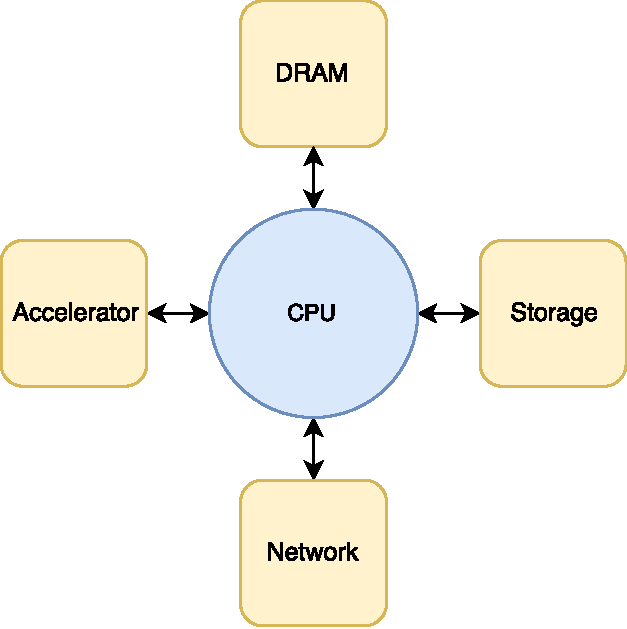
\includegraphics[width=0.90\linewidth]{2-system-1.pdf}
%    \caption{Hypothetical system architecture.}
%    \label{fig:2-system-1}
%  \end{subfigure}
%  \begin{subfigure}{0.5\textwidth}
%    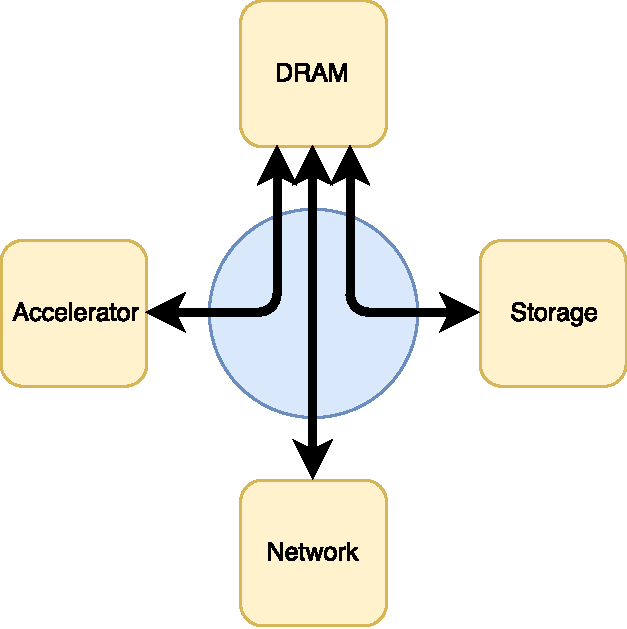
\includegraphics[width=0.90\linewidth]{2-system-2.pdf}
%    \caption{Host memory access congestion.}
%    \label{fig:2-system-2}
%  \end{subfigure}
%  \caption{Hypothetical system architecture suffering from the traditional IO model.}
%  \label{fig:2-system}
%\end{figure}

\begin{figure}[htb!]
\ffigbox[\textwidth]
  {
    \begin{floatrow}
    \ffigbox[\linewidth]
      {\captionof{subfigure}{Hypothetical system architecture.}
      \label{fig:2-system-1}}
      {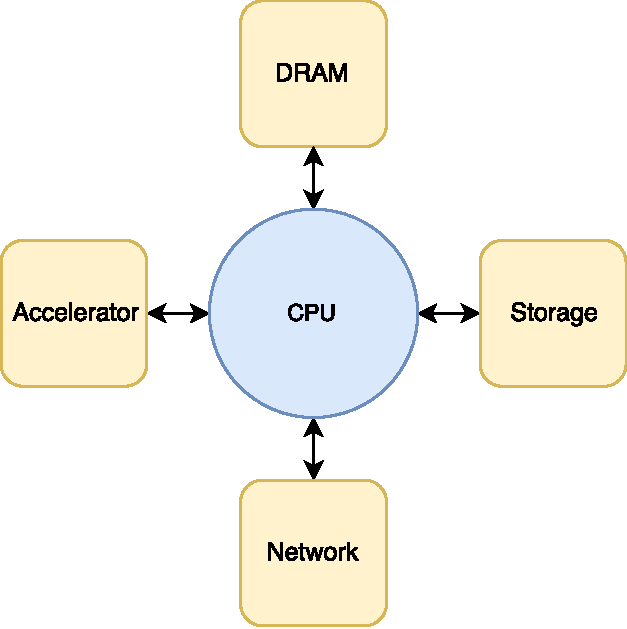
\includegraphics[width=0.8\linewidth]{2-system-1.pdf}}
    \ffigbox[\linewidth]
      {\captionof{subfigure}{Host memory access congestion.}
      \label{fig:2-system-2}}
      {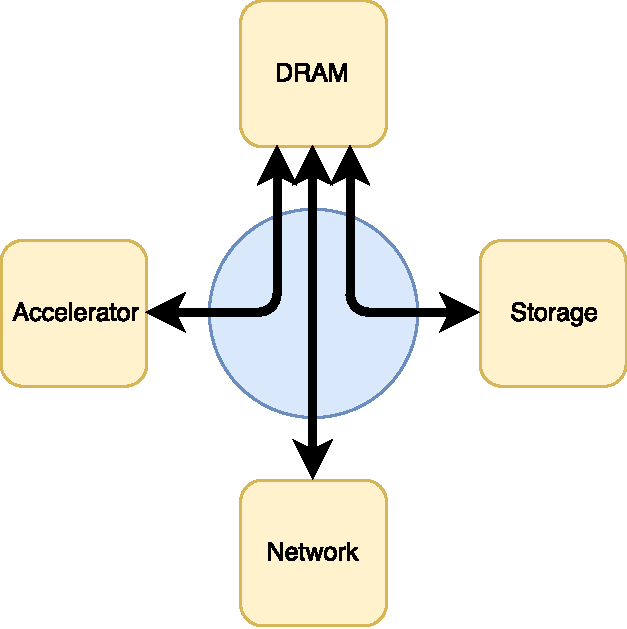
\includegraphics[width=0.8\linewidth]{2-system-2.pdf}}
    \end{floatrow}%
  }
  {\caption{Hypothetical system architecture suffering from the traditional IO model.}\label{fig:2-system}}
\end{figure}





\subsubsection{Case Study: AMD EPYC}
Systems that heavily rely on interconnect bandwidth to improve performance by attaching FPGAs, GPUs, network and storage have to take care that DRAM bandwidth will not become a bottleneck. As shown in Section \ref{sec:bw-trends}, vendors make sure that DRAM bandwidth will not become a bottleneck in the overal system architecture.\\
%Intel's latest generation for example has a DRAM and duplex interconnect bandwidth of \SI{128}{\giga\byte\per\second} and \SI{96}{\giga\byte\per\second} respectively. With a traditional IO model is used, and it probably is, the bottleneck should not be very severe.\\
%IBM's POWER9 processor has a DRAM and duplex interconnect bandwidth of \SI{230}{\giga\byte\per\second} and \SI{492}{\giga\byte\per\second} respectively, where most IO employs a shared memory approach. With the absence of a shared memory space, the DRAM bandwidth would seriously limit system performance.\\
In contrast, AMD's EPYC processor has a DRAM and duplex interconnect bandwidth of \SI{170}{\giga\byte\per\second} and \SI{256}{\giga\byte\per\second}, respectively. Since PCI Express Gen 3 is used, it could very well be that a traditional IO model is used since PCI Express Gen 3 does not support a shared address space between the processor cores and attached devices. If this is the case, system performance could be seriously limited. However, half of the PCI Express Gen 3 lanes can be used for SMP, and this way would remove the bottleneck.





\section{Interconnect Coherency and Shared Memory: A Necessity}
\label{sec:trends-interconnect}
Recent initiatives target the limitations described in Section \ref{sec:current}. Current widely adopted interconnect standards such as PCI Express and AXI are based on the traditional IO model. However, extensions try to improve the usage model. Chapter \ref{ch:state} will discuss the state-of-the-art interconnects in more detail. This section explores necessary changes to the traditional IO model to accommodate for the bandwidth scaling employed by current and future processors.



\subsection{Coherent IO Model}
In order to continue scaling of IO bandwidth to fulfill the requirements of emerging accelerators and attached devices, the traditional IO model has to change and the bottlenecks presented in Section \ref{sec:current} have to be addressed.\\
Shared memory and coherency should be extended to attached devices since accelerators will become an integral part of the ecosystem and should act as a peer to processor cores. System memory should be relieved from performing data copies by employing a shared memory address space between the processor cores and attached devices. Coherency will simplify the programming model for attached devices. Communication overhead can be improved by allowing for shared variables between the host and the attached device in shared memory.\\
The coherent IO model is shown in \autoref{fig:2-desired}. In comparison to the traditional IO model, shown in \autoref{fig:2-memcpy}, there is no CPU involvement and no longer any driver overhead, since copying to buffers is not required. The application has direct access to the address space of the attached device and data exchange is coherent.

\begin{figure}[h]
  \centering
  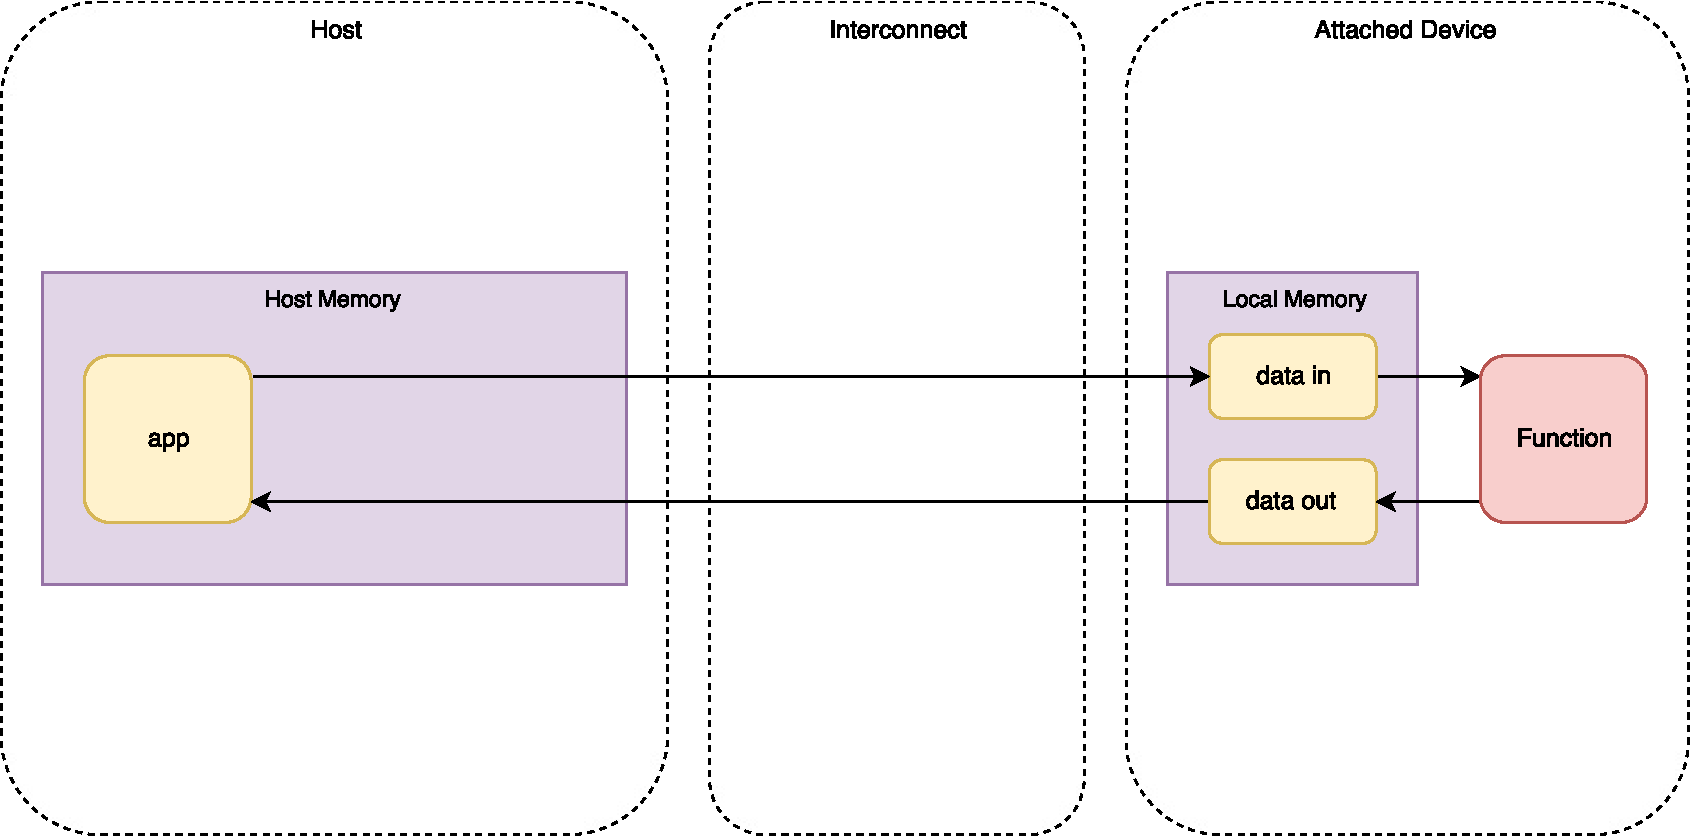
\includegraphics[width=0.80\textwidth]{2-desired.pdf}
  \caption{Coherent IO model.}
  \label{fig:2-desired}
\end{figure}

With the coherent IO model, attached devices are no longer notified using MMIO communication but instead using shared memory. Similarly, completion by the attached device is signaled using shared memory instead of an interrupt for example. By using shared memory, device driver and operating system overhead is decreased significantly.\\
In comparison to \autoref{fig:2-system}, the coherent IO model not only removes the memory copy overhead and therefore avoids memory access congestion, it also allows attached devices to move data between each other without touching host memory. An example could be that data is coming in through a network controller and is immediately moved to an accelerator, as shown in \autoref{fig:2-system-3}.\\
The following sections discuss the required changes for the coherent IO model in more detail.

\begin{figure}[h]
  \centering
  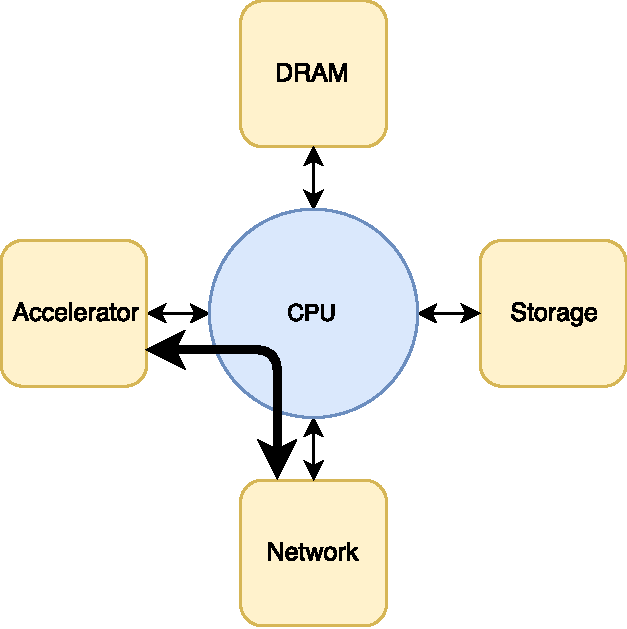
\includegraphics[width=0.4\textwidth]{2-system-3.pdf}
  \caption{Hypothetical system architecture with a coherent IO model.}
  \label{fig:2-system-3}
\end{figure}



\subsection{System-Wide Shared Memory Address Space}

%\todo{- [Extra] What is required in hardware/software for a shared memory address space to work?\\
%}

%\todo{PETER call 29 December. Shared memory and coherence:\\
%- Peter didn’t see this before: key reason for shared memory. if you don’t have shared memory, data structures look different, depending on if host cpu executes it or if accelerator execute it.

%— what do you mean by that? (Yvo asked)\\
%because acc that does not work on coherence memory can’t dereference a pointer. that means that if i have some gigantic piece of code and in the middle i have a function that i want to acc, but i cant, if i want to put it on an acc with PCI Express, i have must make sure i resolve every reference, because acc cant. may not even be possible at compile time to resolve pointers.\\
%to me, its a lot about ease of programming (middle piece of code example; if you have a big piece of code and in the middle you want to accelerate something, you can do that fairly easily with (open)capi. traditional accelerators need more work), in exceptional case where acc has to dereference pointer, it can, just like a thread.
%only thing you have to do, for acc you cant pass arguments through regs. If I am calling a function, here every parameter is on the stack.

%If I am calling a function then, basically if you put all arguments on the stack, then when you call a function the only thing you need to give it is the stack pointer. these days with large reg files, people have calling conventions where a bunch of parameters are also in registers.\\
%if you want to acc with a CAPI attached device, it cant fetch private registers. you have to put all your args on the stack, then you can call an FPGA and act similarly to a thread on a CPU.\\
%no massive restructuring of code, depending on your underlying hardware. very little difference between thread and accelerator. Results in portable code!
%}

Shared memory is an abstraction of a system with multiple physical memory resources and presents these memory resources as a continuous address space. It is desired by programmers to hide details of memory accesses from different physical locations. Without shared memory, data structures look different between the host and accelerator because the accelerator is not able to dereference a pointer. All pointers have to be resolved before sending the code to the accelerator for execution, and this may not even be possible.\\
A shared memory address space will decrease congestion of accessing system memory to result in lower access latency and device driver overhead \cite{capi-cantle}. It also improves programmability since it enables shared buffers (zero-copy) and pointer dereferencing, thus simpler data movement between physical memories (host and device memory). The accelerator acts similar to a processor thread and this allows to easily accelerate a single function in a big application, without having to massively restructure the code.\\
It is obvious that interaction with attached devices using the traditional IO model is not perfect. It requires complex drivers on the host, is error prone due to user data movement, and has a high latency rendering it unpractical for latency sensitive workloads. Shared memory allows the system memory address space to be shared with the IO. This enables for example direct data movement from a network card to a GPU, instead of first copying to main memory or interaction by the CPU. This is achieved by providing the IO with the same address translation tables as the CPU.

%\todo{- [Peter] You can also make a programmability/accelerator transparency argument here.}



\subsection{System-Wide Coherence}

%\todo{- What is required in hardware/software for a coherence to work?\\
%- Is there a significant performance gain or does it only simplify the programming model?\\
%- Why does it enable pointer chasing?\\
%- Important for IO cache coherence: Hennessy page 113: I/O cache coherency question. Page 113: Processor cache coherency is a critical subject in the age of multi-core processors, and we will examine it in detail in Chapter 5.\\
%- Does coherency enable lower latency access to memory? Does it do anything for the memcpy problem encountered before?\\
%}



Caches are widely used in microprocessors and cache hierarchies are becoming larger and more complex, by using various cache levels. By scaling the number of processor cores on a single die, multiple copies of the same data can exist. Cache coherency is required to keep data coherent without any software-intervention. Relying on software to provide snooping, write-back, and invalidation is relatively slow. Hardware-based coherence is preferred since it simplifies the programming model and is faster.\\
%(REF: \url{http://compgroups.net/comp.arch/PCI Express-cache-coherent/191462}).\\
Currently, without coherence, the user has to take care of moving data between resources manually, which is error prone. Typically, data is transferred to the accelerator and the application waits for an interrupt signal from the accelerator to signal completion. The application fetches the result from the accelerator across the interconnect. Caches have to be flushed before other resources can access the data. The FPGA feels more like an off-load engine instead of an extension to a thread running on the CPU.\\
With coherency, a consistent view of memory contents by all participants (CPU cores and IO devices) is guaranteed. Attached devices operate natively within the application’s user space and coherently with the host CPU. This allows attached devices to fully participate in an application without kernel involvement or overhead \cite{opencapi-enablement}.\\
With software coherence, a large burden is placed on the application, drivers and OS to manage timed cache cleaning, maintenance and invalidations. Such operations take time and effort (cache contents have to be written out to system memory). Since caches are invisible to software, managing all of these copies in software is difficult. Keeping caches coherent in software means that all caches have to be flushed \cite{axi-coherence}.\\
Hardware coherency removes the software challenges and makes sharing transparent to the application, at the cost of additional memory traffic between caches about the state of their contents in order to keep all of them synchronized.\\
Coherency also enables new types of workloads such as pointer chasing, but is not truly required. It does significantly simplify the programming model by providing synchronization between the host and attached device mechanisms in hardware or software, therefore making slow interrupt-based solutions obsolete.



\subsection{Thread Synchronization}
Before the usage of accelerators and other attached devices was as common as today, multiple processor cores were used to exploit workload parallelism. Such workloads typically make extensive use of synchronization operations such as barriers, mutexes and semaphores. Therefore, when attached devices act as a peer to processor cores, it makes sense to employ similar synchronization operations. By doing so, notifications using interrupts can be avoided and makes porting existing multi-threaded workloads easier. Instead, the host and attached device communicate through shared variables in shared memory \cite{intel-white}.\\
A lock operation could be implemented from which more complex synchronization operations can be built. Recent interconnect standards incorporate more complex atomic operations to replace the lock operations.\\
Another benefit of moving away from interrupt-based synchronization is that the number of hardware interrupt signals no longer limits the number of interrupts, since interrupts are handled using shared memory. This solution scales much better.





\section{Preliminary Concluding Remarks}
Emerging workloads require a change in system architecture. A diversification of compute resources enables speedups not possible with a single type. The adoption of FPGAs is slow due to interconnect limitations and a complex programming model. To address these issues, attached devices are required to be tightly coupled with the host processor at memory-like bandwidths. Currently, this is not the case and interaction with attached devices involves unnecessary overhead. By extending the shared memory space and coherence domain across the interconnect, attached devices act as a peer to the processor cores. This simplifies FPGA acceleration and enables new usage models. Chapter 3 takes a closer look at state-of-the-art interconnect standards and evaluates the current state of the interaction between the host and attached devices.



% More information:
% CUDA used to have pinned functions. Now is able to immediately instantiate a buffer. Also Unified virtual addressing (UVA) is interesting.
% Directly instantiate buffer: https://devblogs.nvidia.com/parallelforall/how-optimize-data-transfers-cuda-cc/
% UVA: http://docs.nvidia.com/cuda/gpudirect-rdma/index.html#basics-of-uva-cuda-memory-management
% UVA: http://docs.nvidia.com/cuda/cuda-c-programming-guide/index.html#um-unified-memory-programming-hd
% cudaMalloc, cudaMemcpy, etc example: http://developer.download.nvidia.com/CUDA/training/GTC_Express_Sarah_Tariq_June2011.pdf
% Important from previous source: Host pointers point to CPU memory. May be passed to/from device code. May NOT be dereferenced in device code. Same holds for device.
% CPU-GPU data flow: https://gamedev.stackexchange.com/questions/66543/cpu-gpu-memory-data-flow

%\todo{
%- Nice to refer back to earlier in intro for moving to SMP and hetereo. Talk first about moving to SMP requires shared memory to share data between threads, each running on a separate physical CPU core (more on page 348 "In both ... address space is shared". Read more around these pages) and cache coherence. Shared memory for SMP (limit to SMP, no DSM) with caches requires cache coherence (page 351 section 5.2); basic protocols are bus snoop, but scales bad, or directory based, but more complex.\\
%- Check "POWER8 CAPI Education What is CAPI x.pdf" slide 23 and more for general benefits of CAPI and therefore this described new system architecture of tighter coupling of accelerators.\\
%- Hennessy: in age of multi-cores, coherency is important.\\
%Page 346 has general multiprocessor approach and memory organization.\\
%Page 348 "The term shared memory associated with both SMP and DSM refers to the fact that the address space is shared."\\
%Page 352: What Is Multiprocessor Cache Coherence?\\
%Page 386: Synchronization: The Basics, such as atomics.\\
%Read 5.10 Concluding remarks.\\
%}

%\todo{
%- Where is the DMA located in the system? On the CPU, every attached device? See Operating Systems/ I/O Systems pdf.\\
%- Does every attached device have a DMA to master the bus? For example, CPU invokes DMA transfer to GPU. When kernel is done, GPU invokes DMA?\\
%- When CPU moves data from system memory to device, will the DMA on the CPU or on the device be used to handle the transfer?\\
%- Why is the entire system memory not visible to memory-mapped IO devices?\\
%- Why is pinned memory visible to memory-mapped IO devices?\\
%}

%\todo{
%- Great slides on PCI Express versus CAPI and need for shared memory: Enabling Coherent FPGA Acceleration - Allan Cantle\\
%- Typically this happens: pin buffers, translate, map DMA, start IO. Source: Peter Dagstuhl slides.\\
%- Onur Mutlu: Typical system nowadays with memory, CPU, DMA, IO (section 2): \url{http://www.pdl.cmu.edu/PDL-FTP/Storage/decoupled-dma_pact15.pdf}\\
%- Typical CPU-IO interaction: \url{https://stackoverflow.com/questions/11355426/gpu-system-memory-mapping}\\
%}

%\todo{
%- (distributed) shared memory (DSM) model, therefore numa model as well\\
%- importance of (cache) coherency / bus snooping for dsm\\
%- Peter - show conventional way, anything you attach, fpga, network, storage, needs to be copied through memory buffer. this is sum of all io bws added together. like 600GB/s. much more than memory bandwidth of 230GB/s. therefore your memory bw will seriously limit your performance.\\
%- Peter - not everything can copy through memory, too much bandwidth from all attached devices. Much faster to go from network to compute resource for example which will use it directly. No copying needed. This is enabled by (Open)CAPI. If you copy everything through memory, there is just not enough bandwidth to service all other interconnects at the same time. CAPI provides shared address space with main memory which enables that this copying is no longer needed. usually you pin everything in buffer in main memory. then device can see the data (device is io mapped). device doesnt have the same translation tables. Check micro50 slides, peter will probably add something about this. coherency has nothing to do with this. how does coherency then impact the total system?\\
%}

%\todo{
%- Main memory in parallel computer is either shared memory or distributed memory - wiki parallel computing.\\
%- In order to speed-up access, we’ve long used caching to store key data closer to the processor than main memory. When multiple CPUs share a common memory space, they can achieve higher performance if they can use hardware to communicate the cached and/or cacheable state of pieces of that memory. By doing this, each CPU can safely work on a portion of a common dataset without having to use slow software semaphores to control access. If CPU A has cached a piece of memory, it can ensure that CPU B does not modify that same memory space or use an out-of-date copy of the data. To better understand cache coherency, let’s look at a commonly used coherence protocol known as MESI, which refers to the four possible states of a cache line: Modified, Exclusive, Shared, or Invalid. source is 'Using CCIX to implement ...'\\
%- Peter question: if FPGA would have HBM mapped into address space for example, would this be a distributed shared memory system?\\
%- Peter question: for shared memory, do you need both hardware and software to enable it? CUDA has unified virtual addressing for example.\\
%- read: Evaluating cache coherent shared virtual memory for heterogeneous multicore chips PDF.\\
%- News: Linux 4.14 supports heterogenous memory management (HMM) \url{https://tweakers.net/nieuws/131775/linux-414-komt-uit-als-volgende-lts-kernel.html}\\
%}

%\todo{
%- Peter: What else is needed for shared memory to work?\\
%- Peter: Do you call this zero-copy?\\
%- Peter: if FPGA has HBM, can you attach that as well to the address space?\\
%- Peter: address are virtual in P9, is it then shared virtual memory?\\
%}

%\todo{
%- shared virtual memory slides: %\url{http://events.linuxfoundation.org/sites/events/files/slides/Shared%20Virtual%20Memory%20%28SVM%29%20in%20Xen.pdf}\\
%- OpenCL 2.0 shared virtual memroy: %\url{https://software.intel.com/en-us/articles/opencl-20-shared-virtual-memory-overview}\\
%- AMD Fusion slides, zero-copy, CPU-GPU memory sharing: %\url{http://developer.amd.com/wordpress/media/2013/06/1004_final.pdf}\\
%- memory sharing; unified address space amongst cpu and accelerators, even hbm on fpga for example.\\
%- POWER9-VUG pdf (page 19) and CAPI demo pdf (page 5) talk about memory sharing\\
%- Zero-copy data transfers allow for moving data without interaction from the CPU. This not only frees up CPU time and resources, but also reduces latency. While several processors have implemented shared memory, only the recently released SNAP framework by IBM for the POWER8 processor implements the hybrid model of computation mentioned earlier Intel has similar plans for their FPGAs.\\
%}

%\todo{
%- Peter: What is the difference between cache and memory coherence? CAPI has cache coherence but OpenCAPI only system memory coherence. How does that work? Probably coherent memory is that atomic ops are available from the attached device to main memory. Coherent cache is a local cache for the attached device which is coherent with main memory data and other caches.\\
%- Peter: show synchronization example? Naive way which doesnt work, then locks (software), then atomics (hardware).\\
%- problem with multi-thread; mutex/sync with lock and atomics using example. Source with mutex/sync example: \url{https://en.wikipedia.org/wiki/Parallel_computing} at header "Race conditions, mutual exclusion, synchronization, and parallel slowdown"\\
%- Today, atomic transactions are supported for synchronization without using an interrupt mechanism. In emerging applications where math co-processing, visualization and content processing are required, enhanced synchronization would enable higher performance. \url{https://www.embedded.com/design/connectivity/4008241/1/PCI-Express-Gen-3-Simplified}\\
%- Peter: Typically bus-snooping doesn't scale well. How is that solved in the P9?\\
%- Lot of info on cache coherence protocols in Quantitative Approach Chapter 5.\\
%- Must check every place there may be a valid copy, results in a snoop.
%- Snoop filters reduce communication by tracking cache contents \url{http://www.arteris.com/hubfs/2016-05-24-arteris-ncore-overview-PDF-FINAL.pdf}\\
%}

% SOFTWARE FOR FPGAS
%The shift from a traditional CPU-only server, to a CPU and GPU server, to a system consisting of CPUs, GPUs and FPGAs forces the current model of computation to change, both in terms of hardware and software. The typical off-load model of computation used in CPU and GPU systems, where highly parallel data-intensive workloads are taken care of by the GPU while the CPU waits, does not scale well with the addition of more heterogeneous accelerators such as FPGAs. A hybrid model is desired where each part of a workload is mapped onto the compute resource that fits the requirements best. The compute resource selection could be based on different requirements such as power efficiency, lowest latency, currently free or under-utilized resources and more.

%\todo{- rethink what i want to say in this section, especially with respect to requirements for improving adoption of accelerators\\
%- Intel-Alterra FPGAs: fpga in package with already hot xeon, what is fpga/xeon performance in terms of heat dissipation (might be much worse compared to loosely coupled fpga, speculation from my side, source would be great. Also bandwidth numbers would be interesting for comparison) limits the size and frequency of such an on-chip FPGA and large accelerators might not even fit. Having high IO for ASICs and FPGAs solves this problem with OpenCAPI 3.0.
%}
%In order to improve integration of FPGA accelerators and fully utilize their potential, coupling using high bandwidth links is crucial. Especially in the hybrid model of computation where algorithms use fine-grain interactions between all compute resources. Currently this high bandwidth link is realized in one of two ways. By acquiring Altera in 2015, Intel plans to use tightly-coupled FPGAs on-?(chip or die) in their Xeon processors. By having the FPGA close to the CPU, a high bandwidth link is used such that the FPGA can act similarly to a functional unit within the CPU to enhance single thread performance. Other companies are adopting loosely coupled FGPA accelerators by using PCI Express interconnect or the upcoming OpenCAPI interconnect. This enables FPGA acceleration for the system as a whole. Indifferent of how the FPGA accelerator is coupled, all companies agree on a coherent, low latency interconnect (ref intel and opencapi).\\
%Besides raw bandwidth, FPGA accelerator adoption is also driven by less programming effort. In order to achieve that, the following two main problems have to be solved.
%\begin{itemize}
%  \item{Enable high-level languages to be converted into HDL to easily exploit FPGA acceleration by non-hardware engineers.}
%  \item{Simplify the programming model by using shared virtual memory.}
%\end{itemize}

%The first problem is addressed by a large number of available compilers and frameworks which convert (parts of) higher-level programming languages to HDL. Examples include MatLab HDL Coder, Xilinx HLS for C, C++ and SystemC, CLaSH for Haskell to HDL, OpenCL for C and C++, Reconfigure for Go to HDL and MyHDL for Python to HDL. The attainable performance of these tools might not achieve similar performance as fully custom FPGA designs.
%The second problem requires hardware changes to the CPU and allows programmers to implicitly move data using pointers. Zero-copy data transfers allow for moving data without interaction from the CPU. This not only frees up CPU time and resources, but also reduces latency. While several processors have implemented shared memory, only the recently released SNAP framework by IBM for the POWER8 processor implements the hybrid model of computation mentioned earlier Intel has similar plans for their FPGAs.

%\todo{Heterogeneous software frameworks:\\
%- maybe say something about different heterogeneous models of computation. then use software frameworks as well. preferably those that allow to program for mixed hardware, like cpu, gpu, dsp, fpga etc\\
%- framework for fpga acceleration: The Xilinx Reconfigurable Acceleration Stack is targeting the markets for machine learning, video transcoding and SQL queries for data analytics. (Source: Xilinx.)\\
%}
